% Dokumentace projektu GAL 2014
% Vendula Poncová, xponco00
% Alena Chernikava, xcerni07

\documentclass[a4paper, 11pt, titlepage, final]{article}[3. prosinec 2011]

\newcommand{\uv}[1]{\quotedblbase #1\textquotedblleft}
\newcommand{\mensi}{$<$}
\newcommand{\vetsi}{$>$}

\usepackage[left=2.5cm,text={16cm, 25cm},top=2cm]{geometry}
\usepackage[czech]{babel}
\usepackage[utf8]{inputenc}
\usepackage[IL2]{fontenc}
\usepackage[dvipdf]{graphicx}
\usepackage{color}

\newcommand{\url}[1]{\textit{#1}}
\begin{document}

%%%%%%%%%%%%%%%%%%%%%%%%%%%%%%%%%%%%%%%%%%%%%%%%%%%%%%%%%%%%%%%%%%%%%%%%%
% titulni strana - DON'T TOUCH! MAGIC!

\begin{titlepage}
\begin{center}

\textsc{
\Large Fakulta informačních technologií 
\medskip\\
Vysoké učení technické v~Brně}

\vspace{\stretch{0.190}}

{\parbox{5cm}{\centering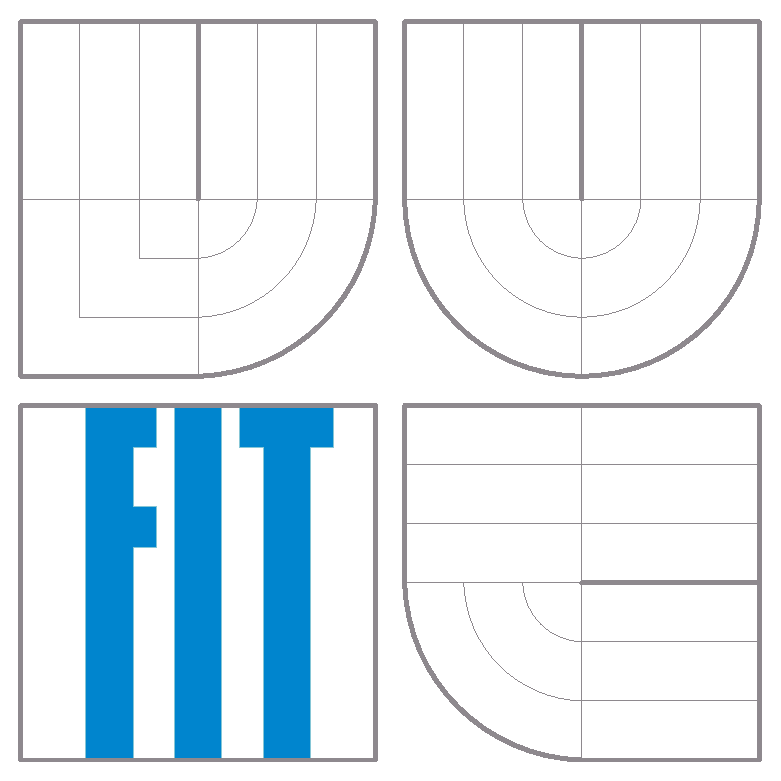
\includegraphics[height=5cm]{img/logo.eps}}}

\vspace{\stretch{0.190}}

{\LARGE Dokumentace projektu do předmětu GAL} \medskip \\
{\Large Paralelizace Egerváryho algoritmu} 


\vspace{\stretch{0.618}}

\end{center}

{\large
Tým 33

Vendula Poncová (\texttt{xponco00})

Alena Chernikava (\texttt{xcerni07})
} \hfill {\large\today}

\end{titlepage}

%%%%%%%%%%%%%%%%%%%%%%%%%%%%%%%%%%%%%%%%%%%%%%%%%%%%%%%%%%%%%%%%%%%%%%%%%
% text dokumentace

\pagenumbering{arabic}
\setcounter{page}{1}

%%%%%%%%%%%%%%%%%%%%%%%%%%%%%%%%%%%%%%%%%%%%%%%%%%%%%%%%%%%%%%%%%%%%%%%%%
\section{Úvod}

%%%%%%%%%%%%%%%%%%%%%%%%%%%%%%%%%%%%%%%%%%%%%%%%%%%%%%%%%%%%%%%%%%%%%%%%%
\section{Egerváryho algoritmus}


\begin{figure}[ht]
  \centering
  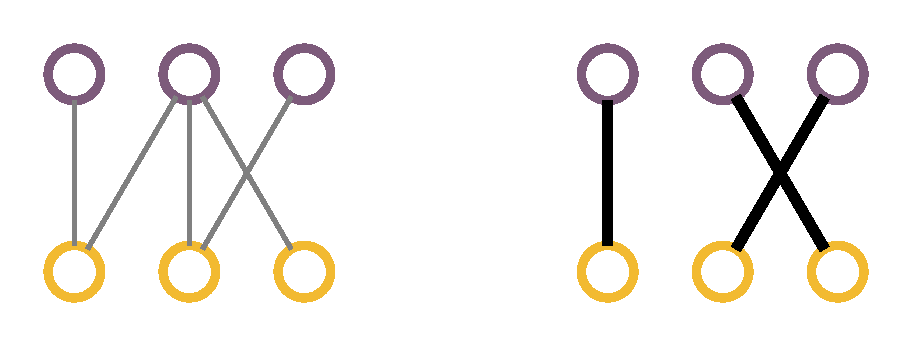
\includegraphics[scale=0.5]{img/bipartite.eps}
  \caption{Bipartitní graf a maximální párování v tomto grafu.}
  \label{imgBipartite}
\end{figure}

\begin{figure}[ht]
  \centering
  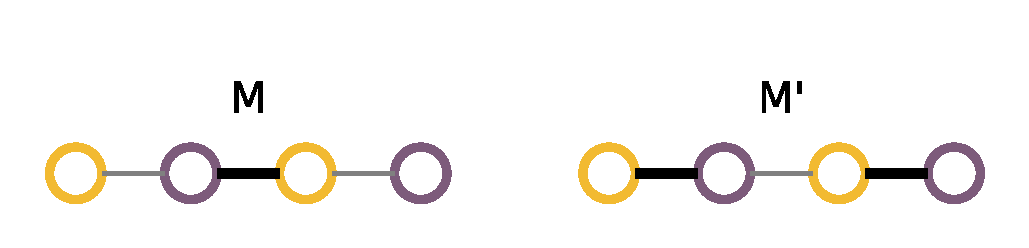
\includegraphics[scale=0.5]{img/mpath.eps}
  \caption{M-rozšiřující cesta a nové párování M'.}
  \label{imgPath}
\end{figure}

\begin{figure}[ht]
  \centering
  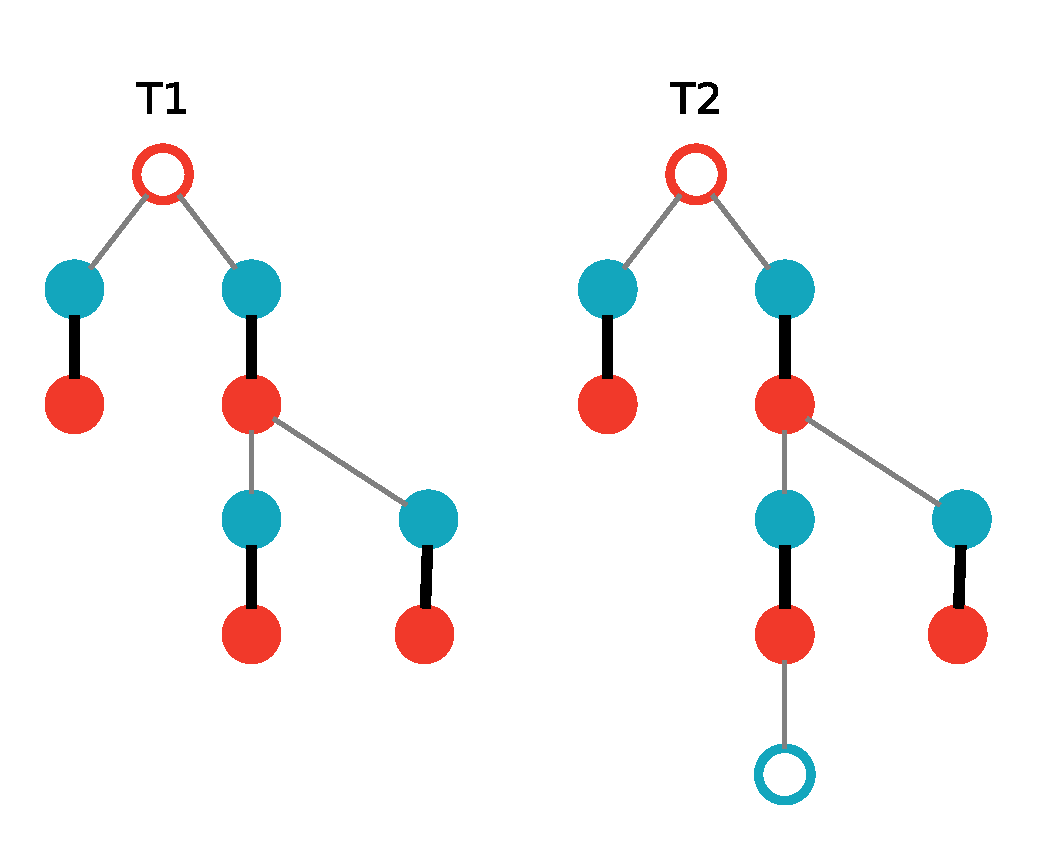
\includegraphics[scale=0.5]{img/trees.eps}
  \caption{M-pokrytý u-strom a M-alternující u-strom.}
  \label{imgTrees}
\end{figure}

%%%%%%%%%%%%%%%%%%%%%%%%%%%%%%%%%%%%%%%%%%%%%%%%%%%%%%%%%%%%%%%%%%%%%%%%%
\section{Sekvenční varianta algoritmu}

\subsection{Datové typy a struktury}

\begin{figure}[ht]
  \centering
  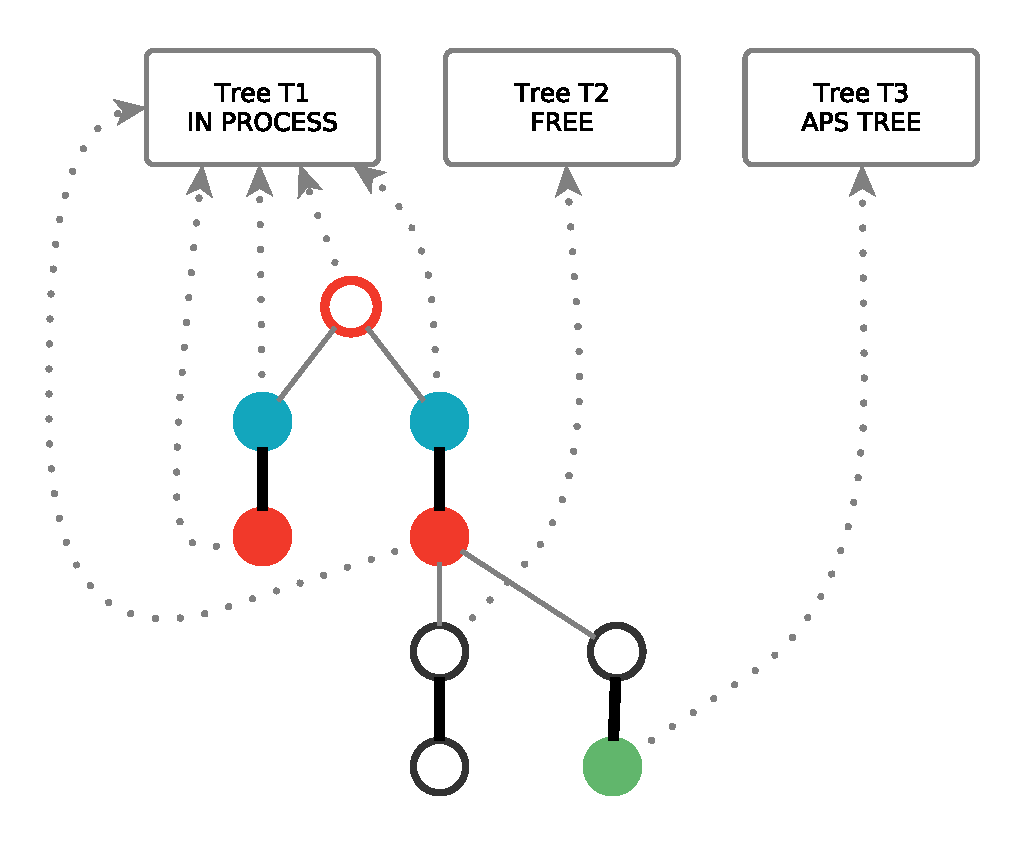
\includegraphics[scale=0.5]{img/implementation.eps}
  \caption{Datové struktury uzlu a stromu.}
  \label{imgStructure}
\end{figure}

\subsection{Popis implementace}


\subsection{Spuštění aplikace}

%%%%%%%%%%%%%%%%%%%%%%%%%%%%%%%%%%%%%%%%%%%%%%%%%%%%%%%%%%%%%%%%%%%%%%%%%
\section{Paralelní varianta algoritmu}

\subsection{Analýza problému}

\begin{figure}[ht]
  \centering
  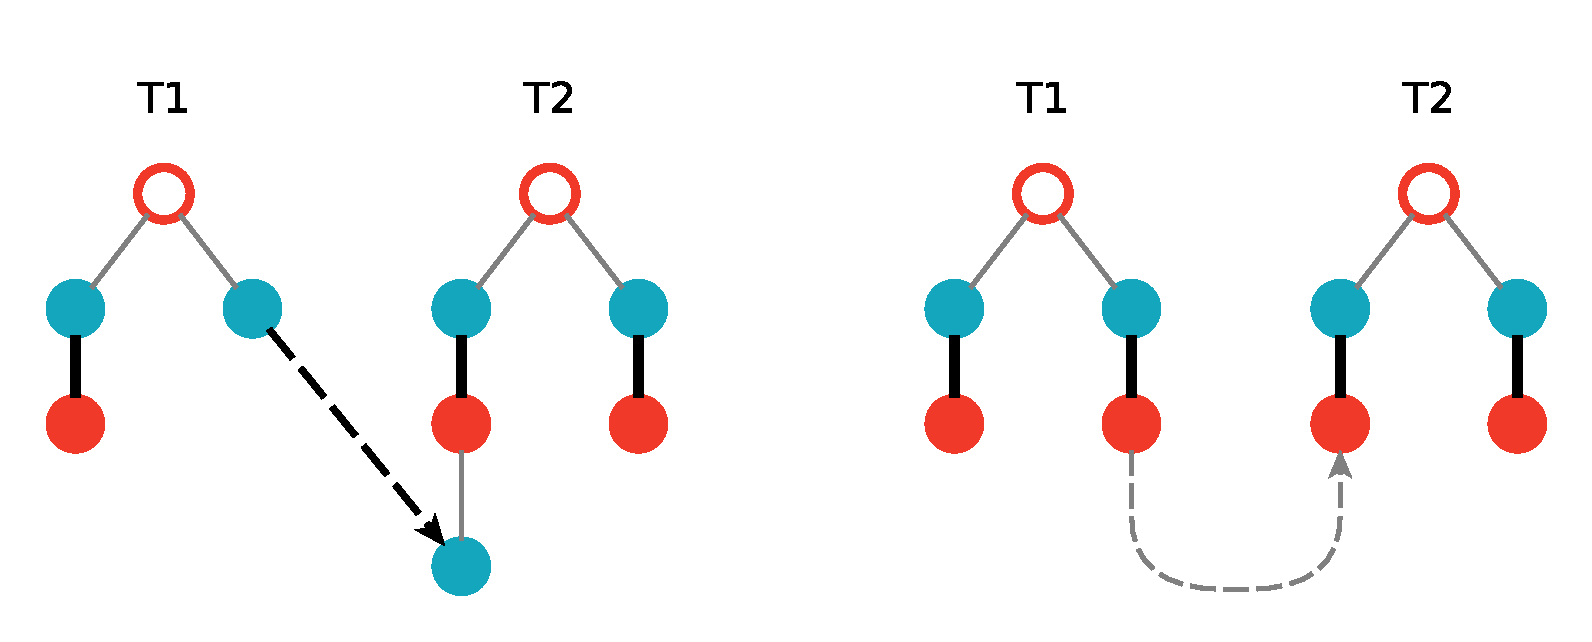
\includegraphics[scale=0.5]{img/XXconflicts.eps}
  \caption{Konflikty B-B a R-R.}
  \label{imgXX}
\end{figure}

\begin{figure}[ht]
  \centering
  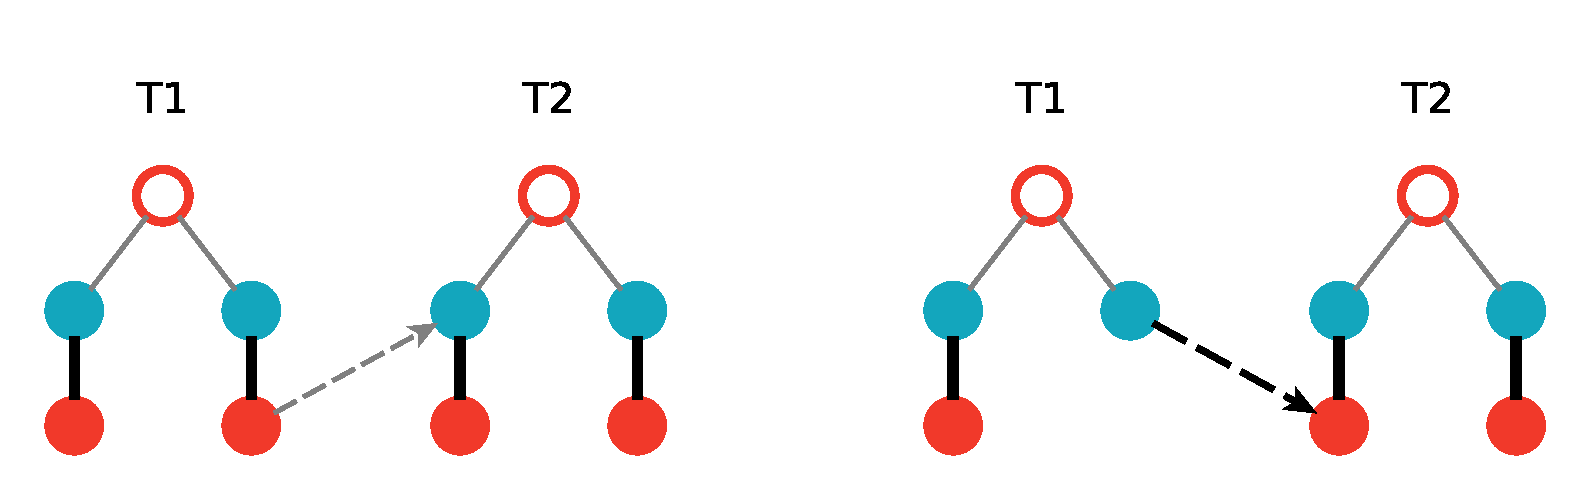
\includegraphics[scale=0.5]{img/XYconflicts.eps}
  \caption{Konflikty R-B a B-R.}
  \label{imgXY}
\end{figure}

\subsection{Návrh řešení}

\begin{figure}[ht]
  \centering
  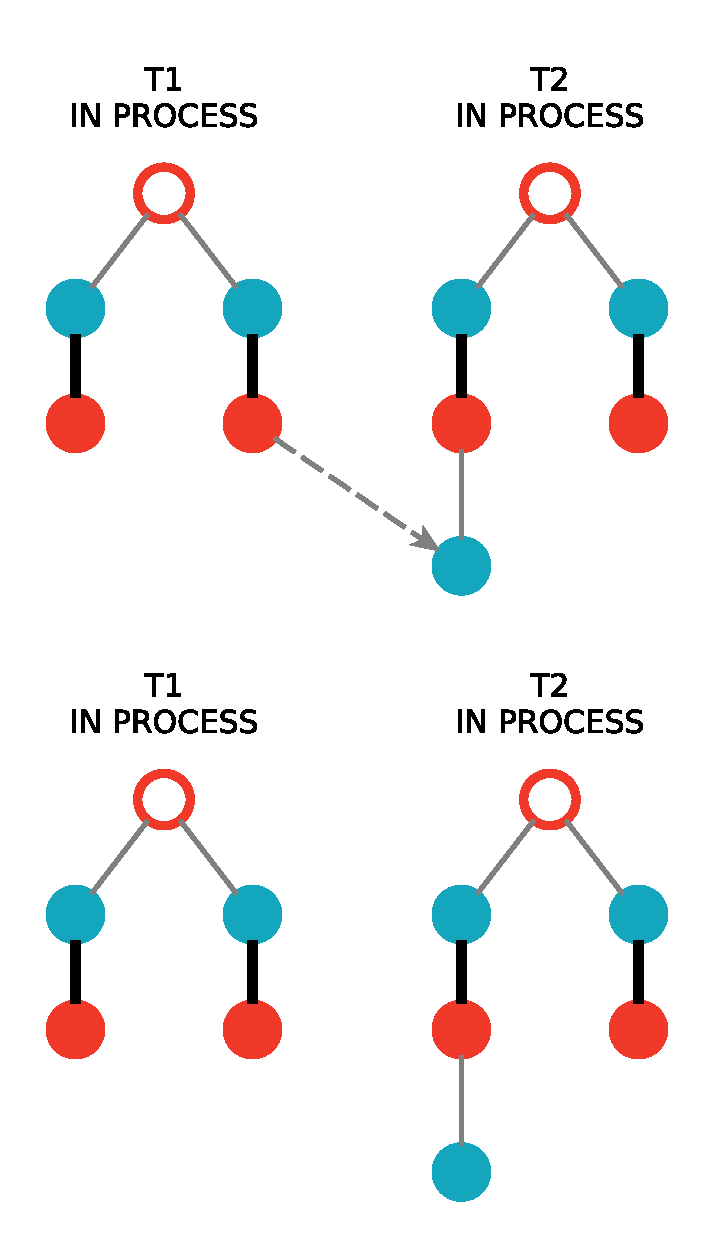
\includegraphics[scale=0.5]{img/inconflict.eps}
  \caption{Řešení R-B konflitu.}
  \label{imgConflict}
\end{figure}

\begin{figure}[ht]
  \centering
  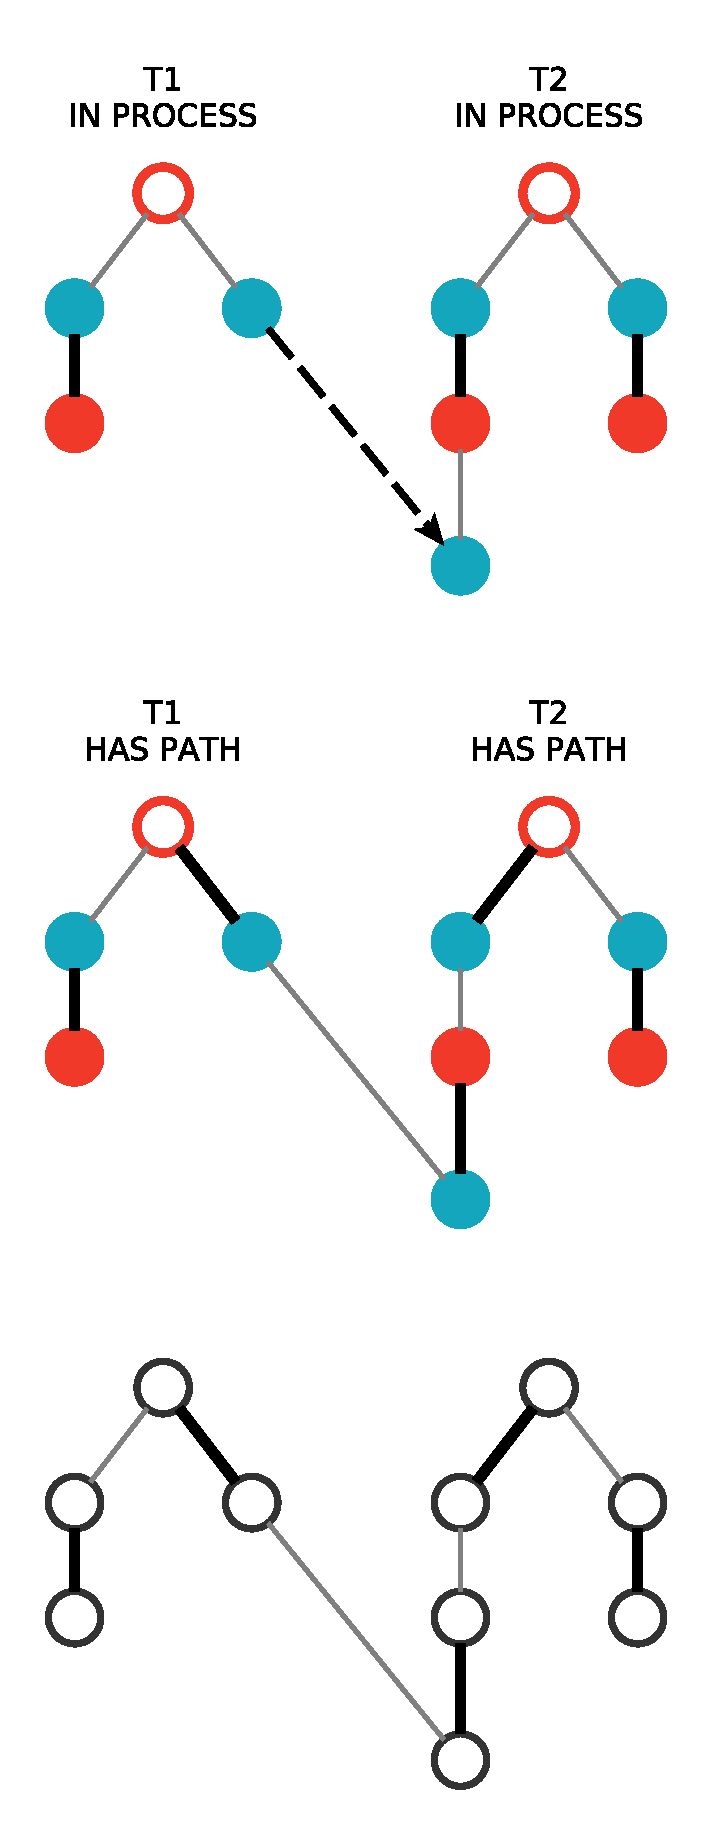
\includegraphics[scale=0.5]{img/haspath.eps}
  \caption{Řešení R-R a B-B konfliktu.}
  \label{imgHasPath}
\end{figure}

\subsection{Datové typy a struktury}

\subsection{Popis implementace}

\subsection{Spuštění aplikace}

%%%%%%%%%%%%%%%%%%%%%%%%%%%%%%%%%%%%%%%%%%%%%%%%%%%%%%%%%%%%%%%%%%%%%%%%%
\section{Experimenty}


%%%%%%%%%%%%%%%%%%%%%%%%%%%%%%%%%%%%%%%%%%%%%%%%%%%%%%%%%%%%%%%%%%%%%%%%%
\section{Závěr}

%------------------------------------------------------------------------
\begin{thebibliography}{1}
  
  \bibitem{bondy:2008} BONDY, J. A. a U. S. R. MURTY. \emph{Graph theory}. New York: Springer, 2008, xii, 651 s. ISBN 978-1-84628-969-9. 

\end{thebibliography}


%------------------------------------------------------------------------
\end{document}

% end of file
